\section{Context}
\label{sec:Context}

\textit{ECCV 2020 : The NERF \cite{mildenhall2020nerf} paper triggers an increasing interest in the field of novel views synthesis}. Can you render novel viewpoints from a given scene using a neural network instead of running a complex ray tracing engine (in a software such as Blender)? The answer is roughly yes and... it also works on real scenes where there's no knowledge of the underlying scene. Many works try to improve the quality/speed of the rendering. We'll see how, suprisingly, point clouds can be used to render novel views of a scene.


\subsection{What is novel view synthesis?}
\label{sec:novel_view_synthesis}


Novel view synthesis is a standard computer vision task which consists in generating new viewpoints of a scene after capturing a set of images.
When taking real photographs of a scene by walking around (or using a drone), the exact pose of the camera is not perfectly known. Even if an inertial measurement unit is attached to the camera which allows later to have an estimation of the camera pose, there will be measurement errors (sensor noise, calibration error, sensor fusion errors). \textit{Please not that efforts can be made, such as calibrating camera/IMU misalignment} \cite*{karpenko2011gyrostab}. 
So there's a need for an algorithm to estimate the camera poses from images, regardless of having an external pose estimation intialization.
The traditional pipeline consists in using Structure from Motion (SfM) like the popular COLMAP software \cite{schoenberger2016sfm} to jointly estimate camera trajectory. A side product of running this algorithm is getting a colored 3D point cloud of the scene. 
The second step is to reconstruct a flexible representation of the scene so it can be rendered from new viewpoint. The technical challenge is to find the most suited data structure to represent the scene subject to constraints such as: 
\begin{itemize}
    \item image / 3D structure quality: for cultural heritage applications for instance. 
    \item reconstruction time and memory consumption. Real time for AR/VR applications is a constraint. \textit{For instance, ADOP seems to take advantage of point cloud rendering hardware acceleration available in any computer using OpenGL (not necessarily with the need of a massive NVidia GPU)}. 
    \item preprocessing time: in case users want to recreate their own scenes, they may not have access to powerful GPU 
\end{itemize}
There's another usecase where the camera poses and scenes are perfectly known and controlled by using 3D scene synthesis. This is an easier setup to study novel view synthesis as you can truly evaluate the rendering quality of the algorithm without doubts on the quality of pose estimation (or camera photometry). This setup is sometimes refered as "calibrated scenes". One could say that representing scenes with sophisticated neural rendering is useless when you have the underlying 3D model and Blender available. Nevertheless, novel view synthesis on calibrated scenes is a good framework to test a method before deploying on real scenes.

\subsection{Representations of the scene}
\label{sec:representations}

If we solely use the colored point cloud, we'll end up with images filled with holes (when we zoom in for instance).
This is where rendering a scene start to get difficult. 
\noindent\textbf{Surface reconstruction.}It is possible to get continuous representations (without holes) by wrapping a surface around the point cloud of an object. For instance assuming we have pre-computed normals, a Signed Distance Function (SDF) defined from point cloud can be evaluated anywhere. The surface of the object is where the SDF is equal to zero. Evaluating IMLS (Implicit Moving Least Square \cite{kolluri2008IMLS}) on a fixed grid followed by the marching cube algorithm allows to recreate a mesh. All topologies may not be represented correctly (e.g. a hole in the cheese may end up being filled).


\begin{figure}[htbp]
    \centering
    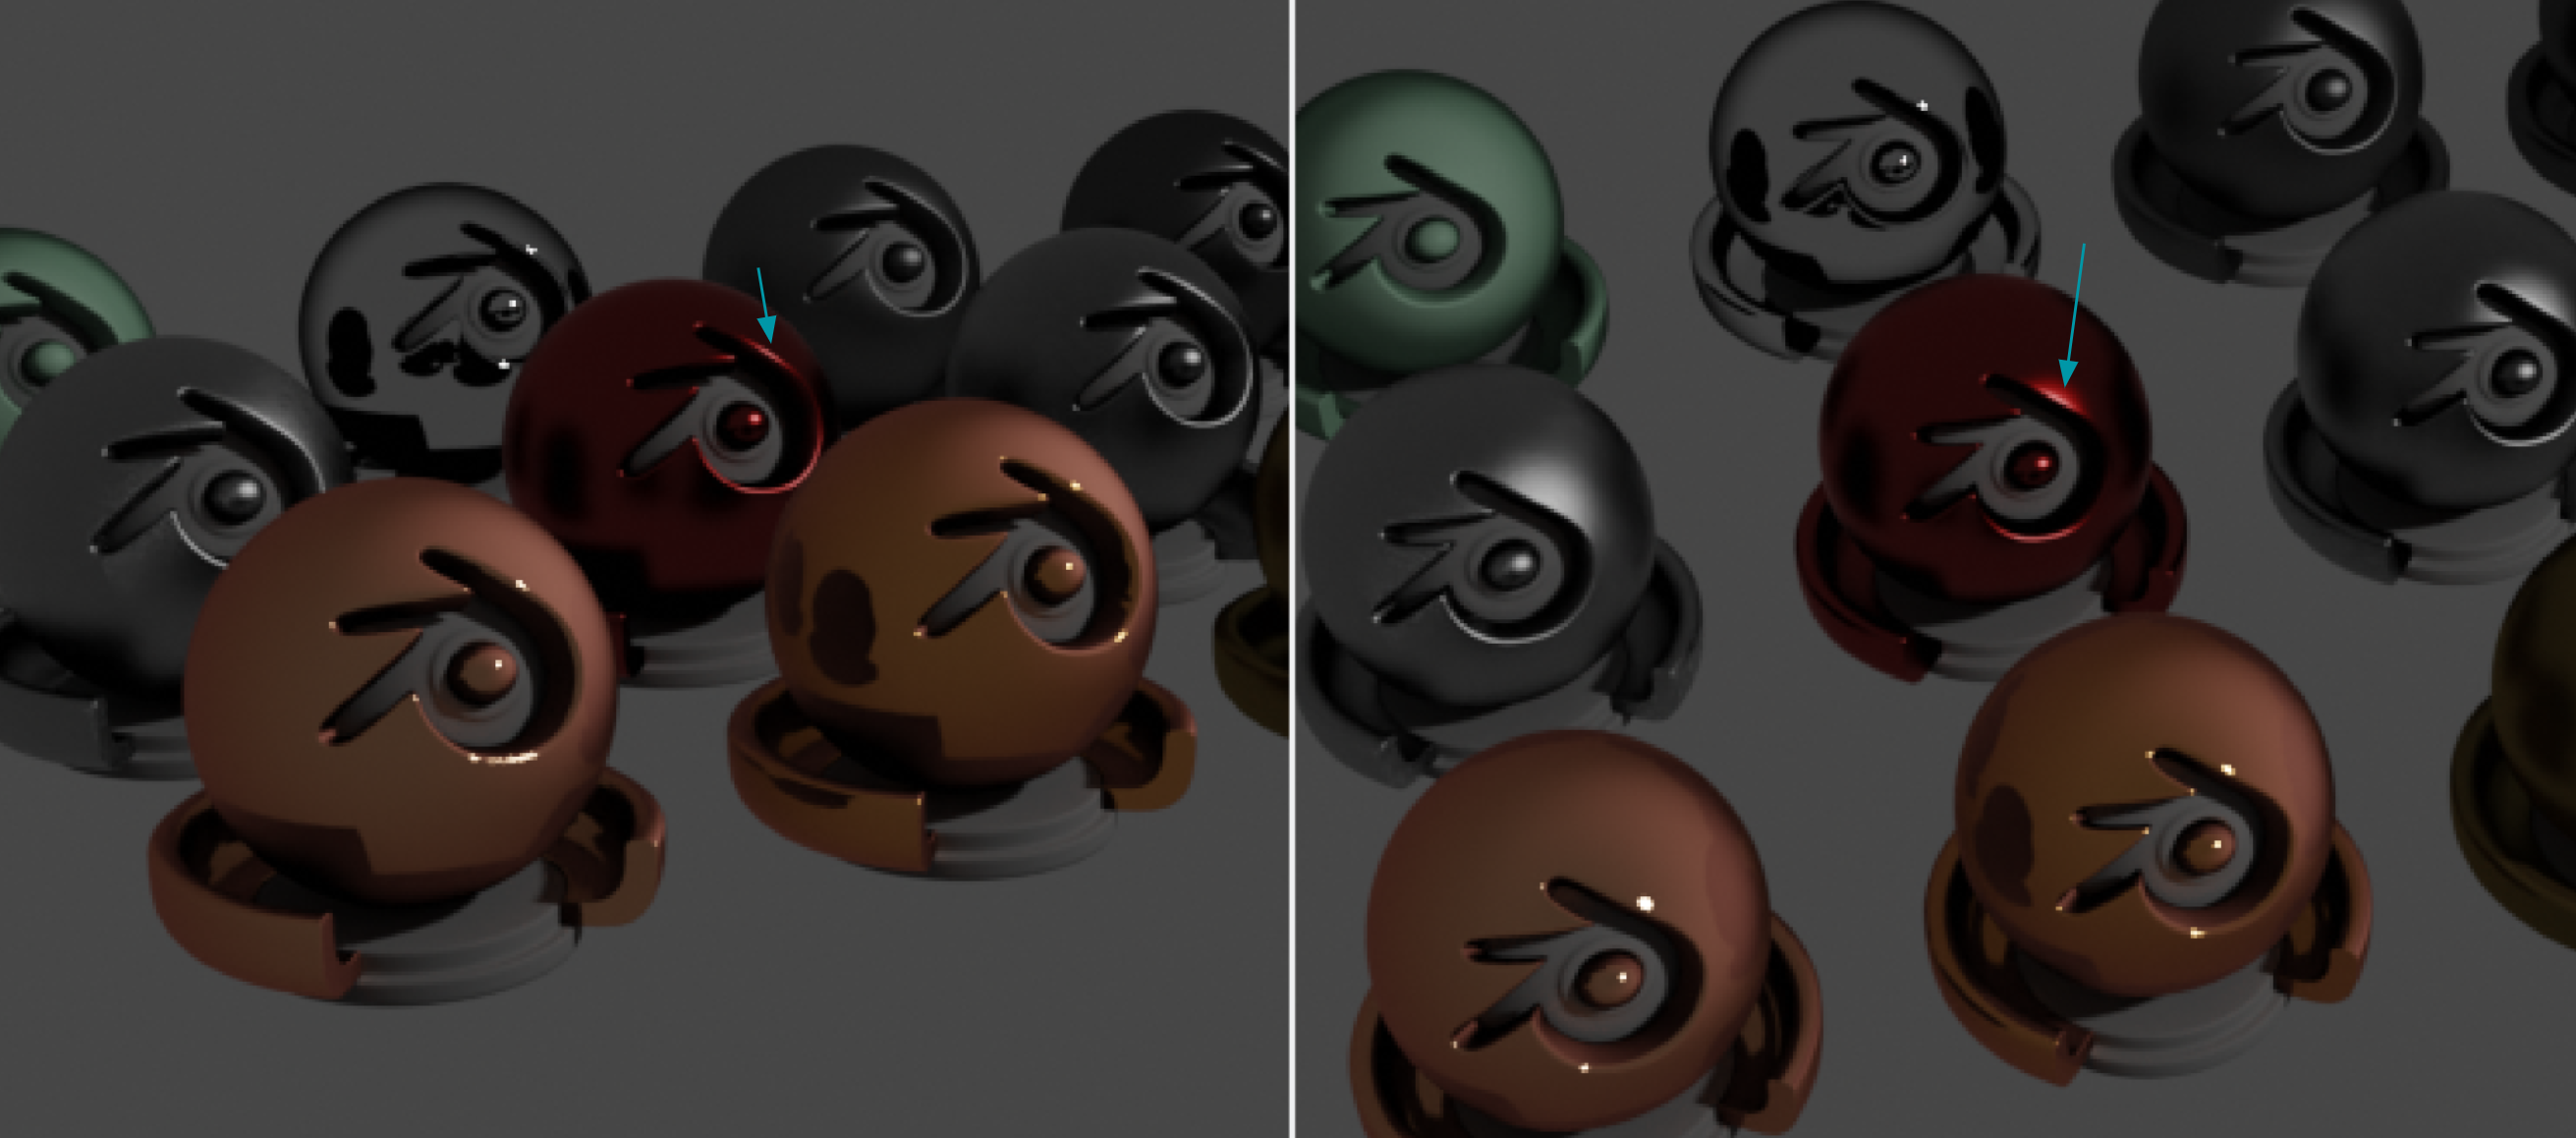
\includegraphics[width=0.5\textwidth]{figures/material_appearance_commented.png}
    \caption{Colors change with camera orientation, specular materials reflect the light and amplify this effect, the extreme use-case being mirrors.}
    \label{fig:material_changes}
\end{figure}

\noindent\textbf{Meshes.} Creating a mesh from the point cloud will lead to a nice geometric representation which can be rendered using classic rasterization techniques. But shading these triangles is still needed. If all materials are perfect diffusers, applying the textures extracted from the photos to the triangles shall be enough. Unfortunately, this will not work for specular materials as illustrated in figure \ref{fig:material_changes}. Neural deferred shading has been proposed \cite{worchel2022nds} to jointly fit a mesh while optimizing a pixel shader (mimicked by a neural network) of a classic mesh rendering pipeline (geometry processing $\rightarrow$ rasterization $\rightarrow$ \textit{(neural)} shader). Please note that the shading is baked into the scene representation and cannot be changed afterwards (for instance, lighting or materials cannot be changed).
\noindent\textbf{Neural radiance fields.} NERF \cite{mildenhall2020nerf} represents the scene colors RGB and density as a function of the 3D position and viewing angle. By shooting rays at the scene, one can integrate the estimated colors to render the final color in the image (density=0 means that the space is empty). A MLP (Multi Layer Perceptron) can approximate basically any function as long as it has enough neurons... here the MLP is used to represent the radiance field. Having the dependance on the viewing angle allows to model complex materials and lighting effects. Main drawback is that NERF are computationally expensive as they require evaluating a MLP all along the rays for each pixel...
\noindent\textbf{Point clouds.} Although point clouds are not continuous, they are a good representation of the scene and kind of easy to manipulate. The introduction of an additional inpainting method (e.g. neural rendering component) in the image space allows to overcome the limitations of the sparseness. These will be discussed in more details the next section on neural point based graphics \ref{subsec:npbg}.



\section{Methodology of the Original Paper}
\label{sec:methodology_paper}

\subsection{Paper overview}
\label{subsec:paper_overview}
ADOP \cite{ruckert2022adop} is a novel view synthesis method based on point cloud representation. 

\noindent\textbf{Geometry.} Pseudo-colors  \footnote{Pseudo-colors means a generic "feature" vector representation which can be more generic than three dimensional RGB components. A dimension 4 for instance.} assigned to each point are projected onto the camera screen at several scales. An environment map is used to model the scene background.

\noindent\textbf{Neural rendering.} The multi-scale pyramid of pseudo images will be jointly decoded and inpainted into a RGB HDR \footnote{We define HDR as high dynamic range linear RGB images - as if they'd been retrieve from a RAW 12 or 14bit sensor with sole operations black point correction, demosaicing and potentially while balance/color matrix transforms.} image at full resolution, using a U-Net architecture.

\noindent\textbf{Camera simulation.} A camera simulation module will transform the image into a LDR image \footnote{LDR stands for low dynamic range images, the ones we see on our screens after tone mapping, color adjustments like vibrancy, vigetting correction etc...}. 

% TODO: ENVIRONMENT MAP!!!!!!!!!!!!!!!!!!!!!!!!!!!!!!!!!!!!!!!!!!!!!
\noindent The whole rendering pipeline is differentiable with regard to:
\begin{itemize}
    \item the pseudo-color of each point
    \item the environment map colors.
    \item the photometry camera parameters (exposure, white balance correction, tone curve parametric vignetting...)
    \item the camera pose and intrinsics \textit{This is an approximation, but it may be useful in order to refine camera pose estimation}. 
\end{itemize}

Using several photos of the scene for supervision, all parameters (network weights, pseudo-colors, environment map and camera photo pipeline) are optimized to minimize a loss function (MSE $\mathcal{L}^{2}$ or perceptual loss\footnote{Perceptual loss \cite{johnson2016perceptual} optimizes the distance between two images in a latent space rather than in the RGB colors space. We usually minimize the $\mathcal{L}^{2}$ distance between the feature maps in the middle of a frozen VGG network}) between predicted LDR rendered images and the real ones. 



\subsection{Neural Point Based Graphics}
\label{subsec:npbg}
NPBG \cite{Aliev2020} (Neural Point-Based Graphics) introduced several important concepts which will be discussed in the next section.
The idea of filling the holes between projected points by using multi-scale convolutional neural networks.  

\subsection{Point based Rendering}
\label{subsec:Point based Rendering}
One of the major advantage of point based methods is that this technology is backed by years of prior industy work. Rendering point clouds can be hardware accelerated and is available to the mainstream public on basically any computer (without NVidia GPU). Libraries such as OpenGL offer the option to render points \texttt{GL\_Points} (and even specify the size of the splat \texttt{glPointSize(1);})... Point clouds can even be rendered in a web browser as shown in figure \ref{fig:potree}.

% https://github.com/rougier/python-opengl/blob/master/07-points.rst
% https://glumpy.github.io/

\begin{figure}[htbp]
    \centering
    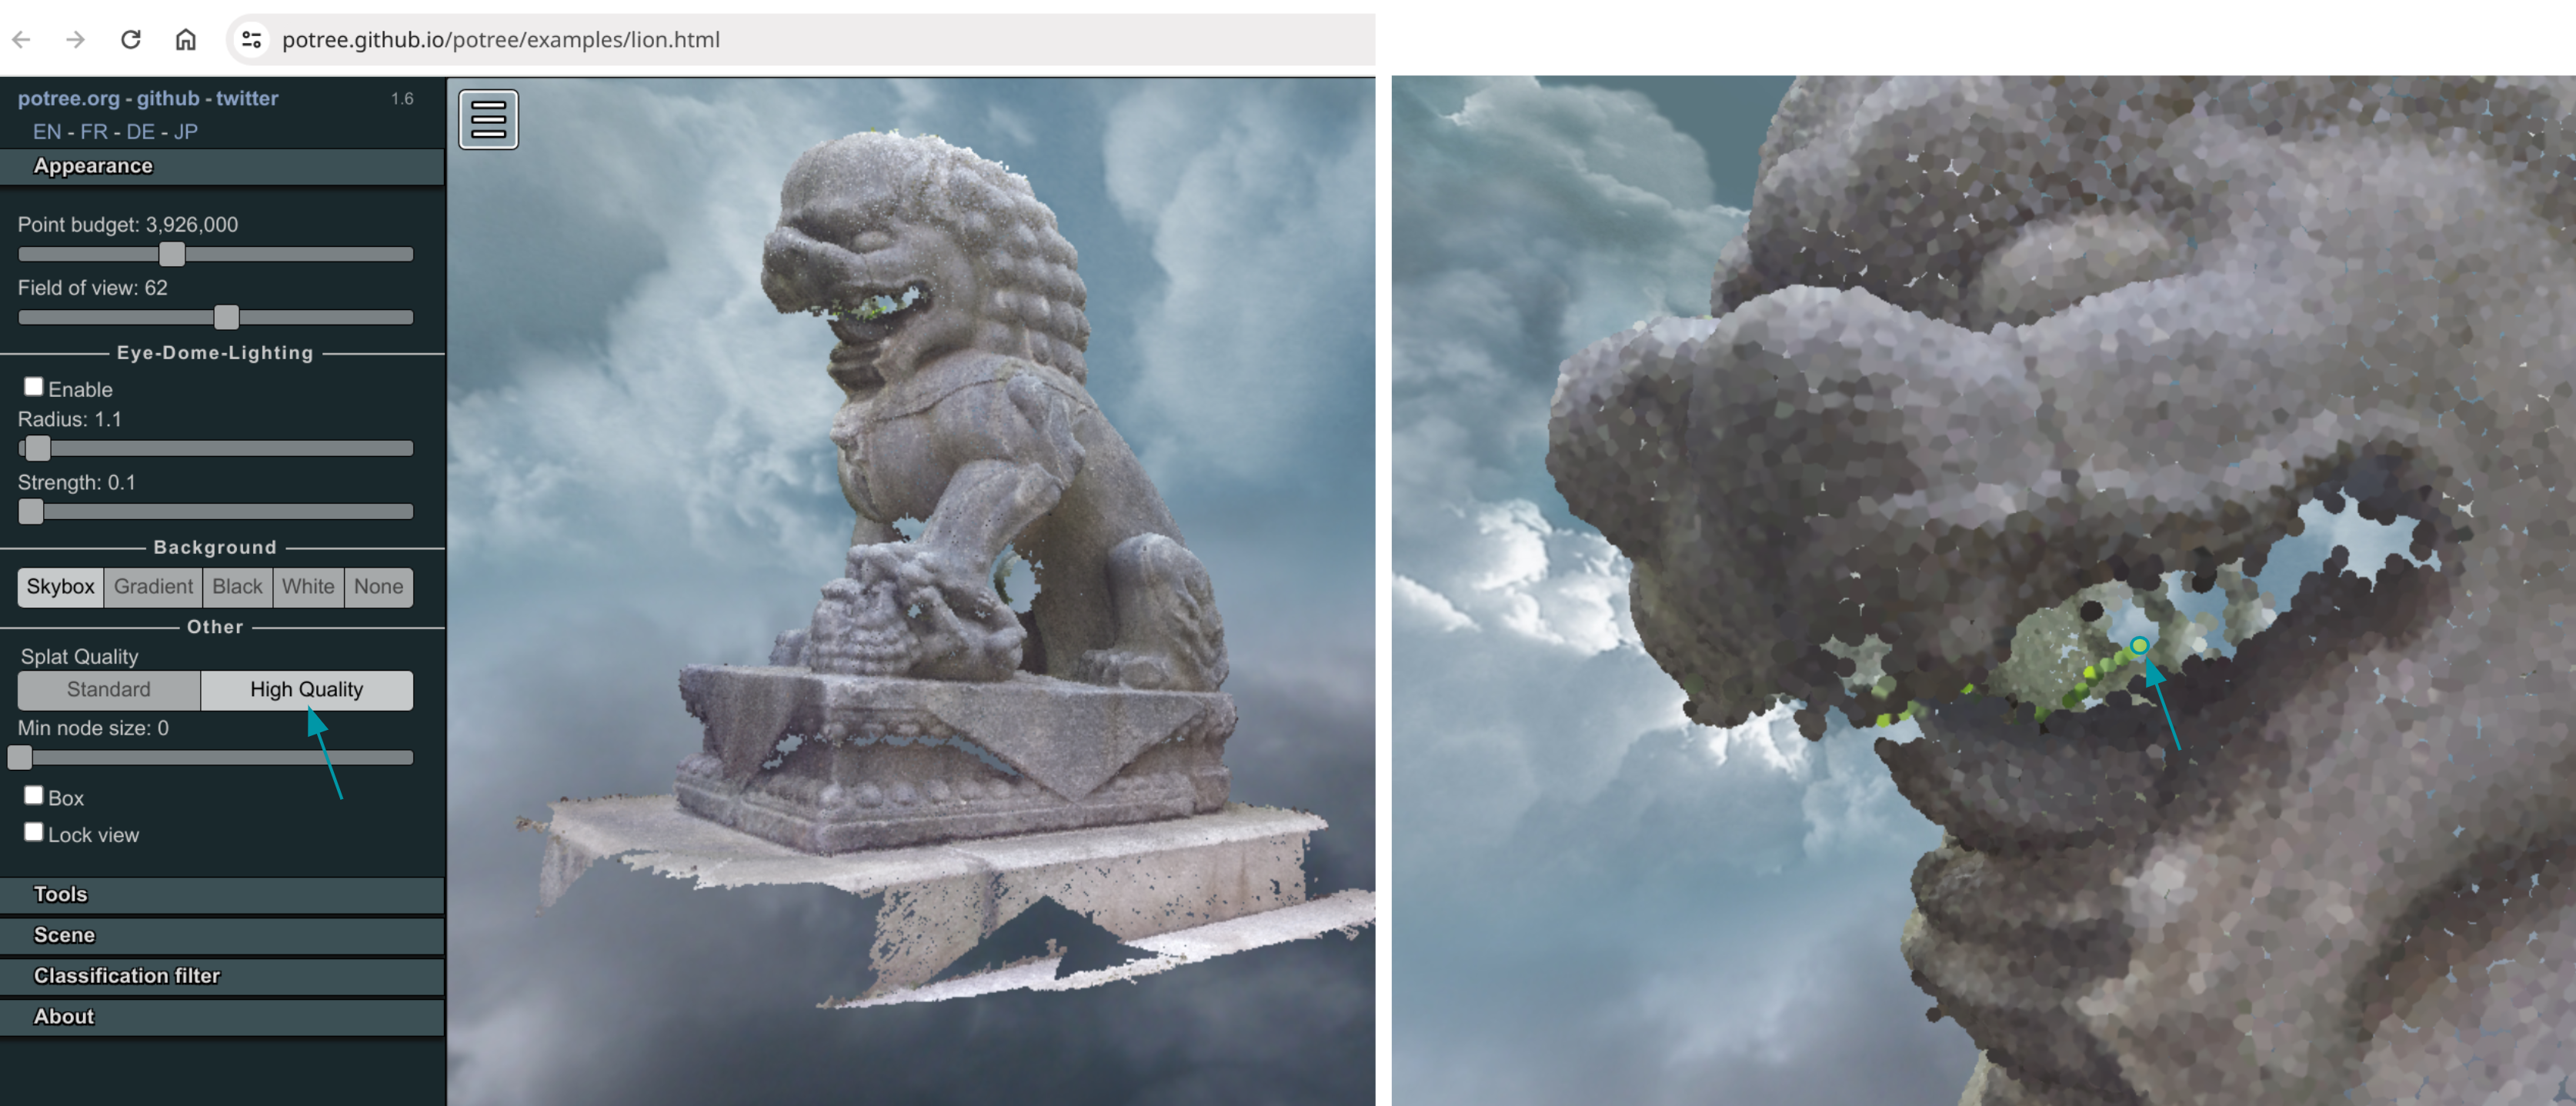
\includegraphics[width=0.5\textwidth]{figures/potree_rendering_and_splat.png}
    \caption{Potree \cite{potree} allows point cloud rendering in the browser, points being rendered as tiny circles splatted on the screen.}
    \label{fig:potree}
\end{figure}



\subsection{Novel view}
\label{subsec:Projecting points}



\noindent\textbf{Implementation.} The authors used lib Torch to compile the code. 

